\documentclass[floatsintext,jou]{apa6}

\usepackage{amssymb,amsmath}
\usepackage{ifxetex,ifluatex}
\usepackage{fixltx2e} % provides \textsubscript
\ifnum 0\ifxetex 1\fi\ifluatex 1\fi=0 % if pdftex
  \usepackage[T1]{fontenc}
  \usepackage[utf8]{inputenc}
\else % if luatex or xelatex
  \ifxetex
    \usepackage{mathspec}
    \usepackage{xltxtra,xunicode}
  \else
    \usepackage{fontspec}
  \fi
  \defaultfontfeatures{Mapping=tex-text,Scale=MatchLowercase}
  \newcommand{\euro}{€}
\fi
% use upquote if available, for straight quotes in verbatim environments
\IfFileExists{upquote.sty}{\usepackage{upquote}}{}
% use microtype if available
\IfFileExists{microtype.sty}{\usepackage{microtype}}{}

% Table formatting
\usepackage{longtable, booktabs}
\usepackage{lscape}
% \usepackage[counterclockwise]{rotating}   % Landscape page setup for large tables
\usepackage{multirow}		% Table styling
\usepackage{tabularx}		% Control Column width
\usepackage[flushleft]{threeparttable}	% Allows for three part tables with a specified notes section
\usepackage{threeparttablex}            % Lets threeparttable work with longtable

% Create new environments so endfloat can handle them
% \newenvironment{ltable}
%   {\begin{landscape}\begin{center}\begin{threeparttable}}
%   {\end{threeparttable}\end{center}\end{landscape}}

\newenvironment{lltable}
  {\begin{landscape}\begin{center}\begin{ThreePartTable}}
  {\end{ThreePartTable}\end{center}\end{landscape}}




% The following enables adjusting longtable caption width to table width
% Solution found at http://golatex.de/longtable-mit-caption-so-breit-wie-die-tabelle-t15767.html
\makeatletter
\newcommand\LastLTentrywidth{1em}
\newlength\longtablewidth
\setlength{\longtablewidth}{1in}
\newcommand\getlongtablewidth{%
 \begingroup
  \ifcsname LT@\roman{LT@tables}\endcsname
  \global\longtablewidth=0pt
  \renewcommand\LT@entry[2]{\global\advance\longtablewidth by ##2\relax\gdef\LastLTentrywidth{##2}}%
  \@nameuse{LT@\roman{LT@tables}}%
  \fi
\endgroup}


\ifxetex
  \usepackage[setpagesize=false, % page size defined by xetex
              unicode=false, % unicode breaks when used with xetex
              xetex]{hyperref}
\else
  \usepackage[unicode=true]{hyperref}
\fi
\hypersetup{breaklinks=true,
            pdfauthor={},
            pdftitle={Integrating analysis code and document preparation : An example Rmarkdown + papaja document},
            colorlinks=true,
            citecolor=blue,
            urlcolor=blue,
            linkcolor=black,
            pdfborder={0 0 0}}
\urlstyle{same}  % don't use monospace font for urls

\setlength{\parindent}{0pt}
%\setlength{\parskip}{0pt plus 0pt minus 0pt}

\setlength{\emergencystretch}{3em}  % prevent overfull lines


% Manuscript styling
\captionsetup{font=singlespacing,justification=justified}
\usepackage{csquotes}
\usepackage{upgreek}



\usepackage{tikz} % Variable definition to generate author note

% fix for \tightlist problem in pandoc 1.14
\providecommand{\tightlist}{%
  \setlength{\itemsep}{0pt}\setlength{\parskip}{0pt}}

% Essential manuscript parts
  \title{Integrating analysis code and document preparation : An example
Rmarkdown + papaja document}

  \shorttitle{Example Rmarkdown document}


  \author{Tom Stafford\textsuperscript{1}~\& Mate Giannadou\textsuperscript{2}}

  % \def\affdep{{"", ""}}%
  % \def\affcity{{"", ""}}%

  \affiliation{
    \vspace{0.5cm}
          \textsuperscript{1} Department of Psychology, University of Sheffield\\
          \textsuperscript{2} Department of Psychosocial Science, University of Bergen  }

  \authornote{
    Correspondence concerning this article should be addressed to Tom
    Stafford, Department of Psychology, University of Sheffield, 1 Vicar
    Lane, Sheffield, S1 2LT, UK. E-mail:
    \href{mailto:t.stafford@sheffield.ac.uk}{\nolinkurl{t.stafford@sheffield.ac.uk}}
  }

  \note{\textcolor{red}{This is an example of a note}}

  \abstract{R is a statistical programming language which is increasingly popular
with psychologists. It can import and process your data, fit statistical
models (from simple t-tests to state of the art such as bayesian
multilevel model fitting). It also makes nice plots. RStudio is a way of
editing R scripts and running R analysis. RMarkdown is a way of using
RStudio to produce documents (e.g.~as webpages, MS Word or PDF). Another
advantage is that you can include R code in your document file - so no
more running your analysis in SPSS and copying the results into your
document (and making errors / forgetting which version of the analysis
you ran etc). This is an example document which integrates all the
functions of Rmarkdown - running analysis, formatting references, etc.
It uses an add-on for Rmarkdown called papaja which helps us make nicely
APA formatted documents}
  




\usepackage{amsthm}
\newtheorem{theorem}{Theorem}
\newtheorem{lemma}{Lemma}
\theoremstyle{definition}
\newtheorem{definition}{Definition}
\newtheorem{corollary}{Corollary}
\newtheorem{proposition}{Proposition}
\theoremstyle{definition}
\newtheorem{example}{Example}
\theoremstyle{definition}
\newtheorem{exercise}{Exercise}
\theoremstyle{remark}
\newtheorem*{remark}{Remark}
\newtheorem*{solution}{Solution}
\begin{document}

\maketitle

\setcounter{secnumdepth}{0}



\section{Introduction}\label{introduction}

You will find it useful to compare the output PDF document with the .rmd
document. This latter item is the thing you edit to produce the PDF.

\subsection{Example Subheading}\label{example-subheading}

Here are some example references in the following sentence. For reviews
of this topic see Wickelgren (1977); Heitz (2014). Here is another
example reference. For example, ignoring speed of response is common in
psychophysics, whereas some domains of cognitive psychology where
high-accuracy is assumed, focus only on response times (e.g. Stafford,
Ingram, \& Gurney, 2011)\footnote{As well as an example of a footnote.},
albeit sometimes after a cursory check that standard null-hypothesis
tests do not reveal significant differences in error-rates.

\section{Method}\label{method}

Rmarkdown also lets us track figure labels, and updates them
automatically. Look! Kittens! Illustrated in Figure
\ref{fig:examplefigurename}.

\begin{figure}

{\centering 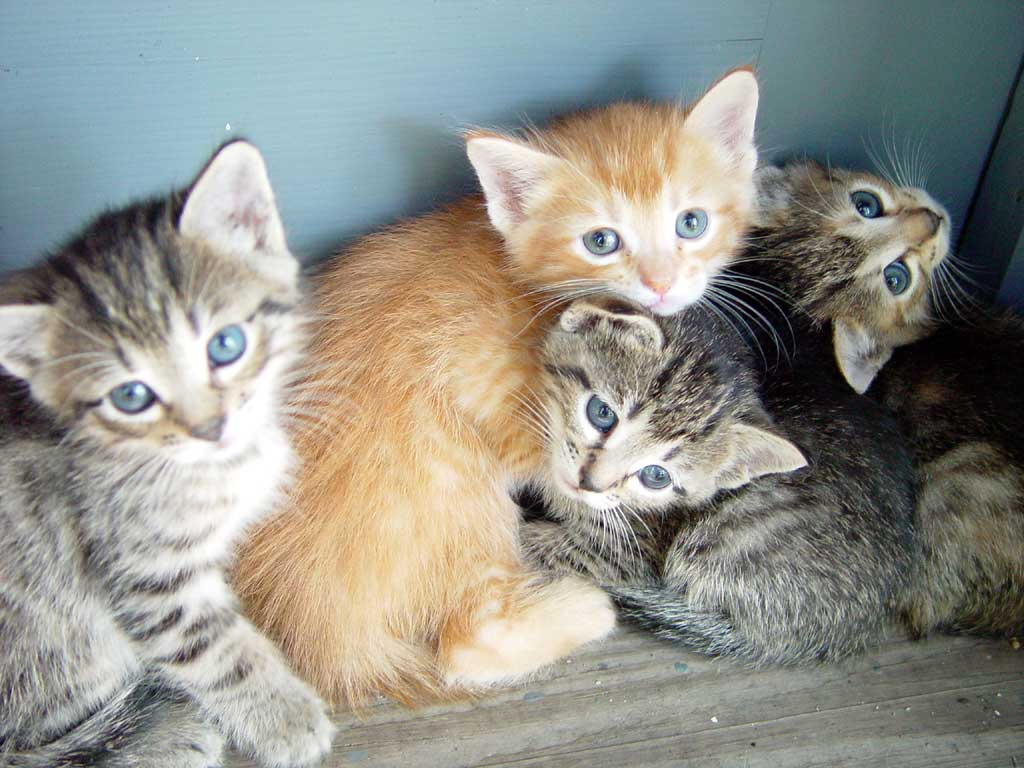
\includegraphics[width=0.75\linewidth]{figs/kittens} 

}

\caption{Example figure caption}\label{fig:examplefigurename}
\end{figure}

\subsection{Requirements}\label{requirements}

You should install R, RStudio and tex and papaja. More details here
\url{https://crsh.github.io/papaja_man/introduction.html\#getting-started}

\section{Results}\label{results}

Now let's integrate some R code to generate/import some data, run and
analyse and integrate it into the document:

You can't see it, but inbetween this paragraph and the last we asked R
to generate some random data and save it to a CSV file. Now we're going
to import the data from the CSV file, as if it was independently created
data - from an experiment or similar - and plot a graph.

\begin{figure}

{\centering 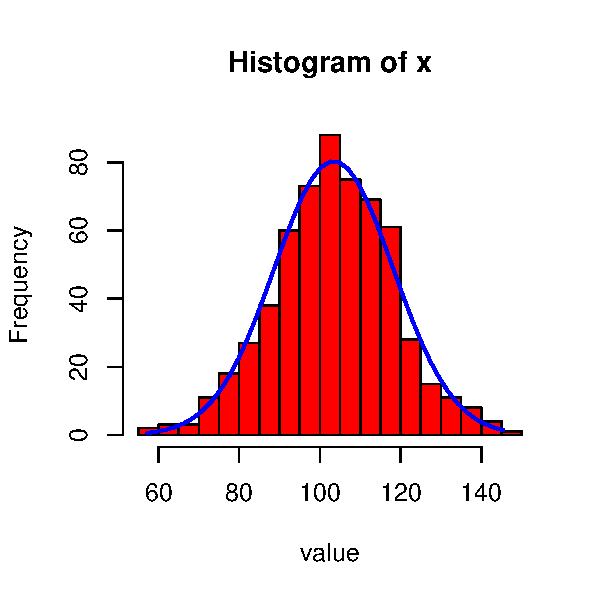
\includegraphics[width=0.75\linewidth]{example_manuscript_files/figure-latex/ourhistogram-1} 

}

\caption{Histogram of all data, grouped}\label{fig:ourhistogram}
\end{figure}

See Figure \ref{fig:ourhistogram}. Of course we could draw all sorts of
things, but this is a proof-of-concept. Finally, let's run a t-test and
integrate the results into the text.

We found there was a statistically significant difference between the
two groups (t=-6.32 (591.61), p = 0.00). Note how the exact values in
the previous sentence change every time we re-make the document (because
the document also re-generates the underlying data).

Unanswered questions: Is this the best way to integrate values into
text? Why is the df not an integer? What is the best way to define
figure sizes so you get nice and/or consistent sizing across document
formats?

\section{Discussion}\label{discussion}

Rmarkdown is good. Need to change reference style? Change one line. Need
to submit as PDF rather than .DOC? Just click \enquote{Word} as output
rather than \enquote{PDF} (instructions here
\url{https://rmarkdown.rstudio.com/articles_docx.html}). Need to change
to two column style to make a nice pre-print? Again, simple - just
change one line!

\subsection{Main conclusions}\label{main-conclusions}

Of course, there's more effort in installing and learning and correctly
marking up your document in the first place, but it is worth it

\section{Acknowledgements}\label{acknowledgements}

This is an example acknowledgements section

\section*{References}\label{references}
\addcontentsline{toc}{section}{References}

\hypertarget{refs}{}
\hypertarget{ref-heitz2014speed}{}
Heitz, R. P. (2014). The speed-accuracy tradeoff: History, physiology,
methodology, and behavior. \emph{Frontiers in Neuroscience}, \emph{8},
150.

\hypertarget{ref-stafford2011pieron}{}
Stafford, T., Ingram, L., \& Gurney, K. N. (2011). Piéron's law holds
during stroop conflict: Insights into the architecture of decision
making. \emph{Cognitive Science}, \emph{35}(8), 1553--1566.

\hypertarget{ref-wickelgren1977speed}{}
Wickelgren, W. A. (1977). Speed-accuracy tradeoff and information
processing dynamics. \emph{Acta Psychologica}, \emph{41}(1), 67--85.






\end{document}
